\documentclass{standalone}
\usepackage{tikz}
\usepackage{ctex,siunitx,ninecolors}
\setCJKmainfont{Noto Serif CJK SC}
\usepackage{tkz-euclide}
\usepackage{amsmath}
\usetikzlibrary{patterns, calc}
\usetikzlibrary {decorations.pathmorphing, decorations.pathreplacing, decorations.shapes}
\begin{document}
\small
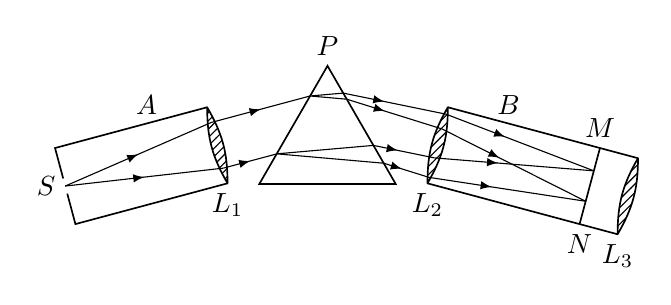
\begin{tikzpicture}[>=latex,scale=1.0]
  % \useasboundingbox(-1,1.2)rectangle(5,2.8);
  \coordinate (A) at ([shift=(-165:1)]150:0.5);
  \coordinate (B) at ([shift=(-15:1)]30:0.5);
  \coordinate (C) at ([shift=(-15:2.5)]B);
  \coordinate (D) at ([shift=(-15:2.0)]B);
  \coordinate (E) at ([shift=(-165:2.0)]A);

  \draw[semithick](90:1)node[above]{$P$}--(210:1)--(-30:1)--cycle;
  \draw[pattern=north east lines,line join=round,semithick]([shift=(105:0.5)]A)to[bend left=15]([shift=(-75:0.5)]A)node[below]{$L_1$}to[bend left=15]([shift=(105:0.5)]A)--cycle;
  \draw[semithick]([shift=(105:0.5)]A)--++(-165:2.0)--++(-75:0.4)([shift=(-75:0.5)]A)--++(-165:2.0)--++(105:0.4);
  \draw[pattern=north east lines,line join=round,semithick]([shift=(75:0.5)]B)to[bend left=15]([shift=(-105:0.5)]B)node[below]{$L_2$}to[bend left=15]([shift=(75:0.5)]B)--cycle;
  \draw[pattern=north east lines,line join=round,semithick]([shift=(75:0.5)]C)to[bend left=15]([shift=(-105:0.5)]C)node[below]{$L_3$}to[bend left=15]([shift=(75:0.5)]C)--cycle;
  \draw[semithick]([shift=(75:0.5)]B)--([shift=(75:0.5)]C)([shift=(-105:0.5)]B)--([shift=(-105:0.5)]C)([shift=(75:0.5)]D)node[above]{$M$}--([shift=(-105:0.5)]D)node[below]{$N$};
  \draw[postaction={decorate},decoration={markings,mark=at position 0.5 with {\arrow{>}}}](E)--([shift=(105:0.3)]A);
  \draw[postaction={decorate},decoration={markings,mark=at position 0.5 with {\arrow{>}}}]([shift=(105:0.3)]A)--(-0.2209,0.6174);
  \draw[postaction={decorate},decoration={markings,mark=at position 0.5 with {\arrow{>}}}](E)--([shift=(-75:0.3)]A);
  \draw[postaction={decorate},decoration={markings,mark=at position 0.5 with {\arrow{>}}}]([shift=(-75:0.3)]A)--(-0.6415,-0.1174);
  \draw(0.1996,0.6542)--(-0.2209,0.6174)--(0.2444,0.5767)(0.5831,-0.0100)--(-0.6451,-0.1174)--(0.7138,-0.2363);
  \draw[postaction={decorate},decoration={markings,mark=at position 0.4 with {\arrow{>}}}](0.1996,0.6542)--(1.5049,0.3865);
  \draw[postaction={decorate},decoration={markings,mark=at position 0.4 with {\arrow{>}}}](1.5049,0.3865)--([shift=(75:0.2)]D);
  \draw[postaction={decorate},decoration={markings,mark=at position 0.4 with {\arrow{>}}}](0.5831,-0.0100)--(1.3561,-0.1685);
  \draw[postaction={decorate},decoration={markings,mark=at position 0.4 with {\arrow{>}}}](1.3561,-0.1685)--([shift=(75:0.2)]D);
  \draw[postaction={decorate},decoration={markings,mark=at position 0.4 with {\arrow{>}}}](0.2444,0.5767)--(1.4545,0.1986);
  \draw[postaction={decorate},decoration={markings,mark=at position 0.4 with {\arrow{>}}}](1.4545,0.1986)--([shift=(-105:0.2)]D);
  \draw[postaction={decorate},decoration={markings,mark=at position 0.4 with {\arrow{>}}}](0.7138,-0.2363)--(1.2898,-0.4163);
  \draw[postaction={decorate},decoration={markings,mark=at position 0.4 with {\arrow{>}}}](1.2898,-0.4163)--([shift=(-105:0.2)]D);
  \node at (-2.3,0.5) {$A$};
  \node at (2.3,0.5) {$B$};
  \node at (E) [left] {$S$};
\end{tikzpicture}
\end{document}